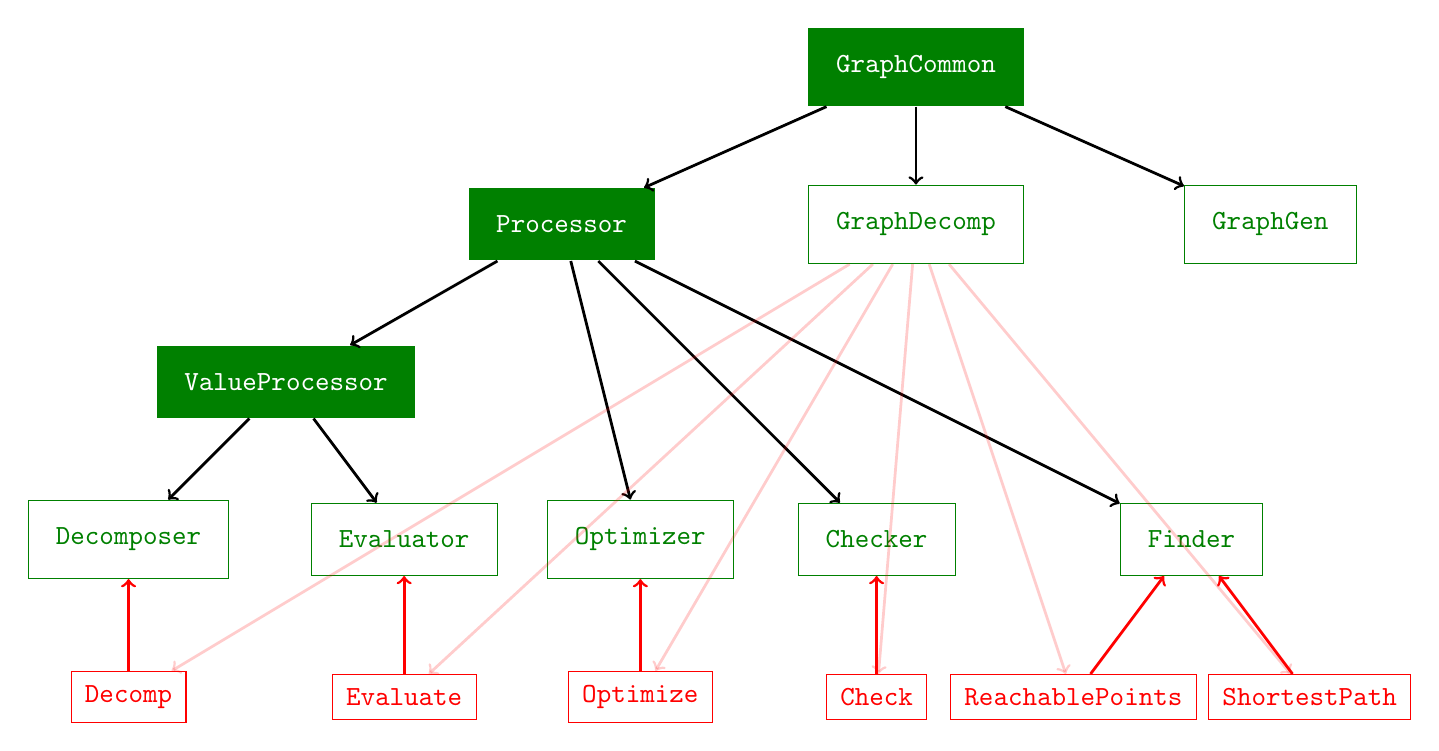
\begin{tikzpicture}
\tikzstyle{class} = [font=\ttfamily\bfseries,color=white,fill=green!50!black,inner sep=10];
\tikzstyle{struct} = [font=\ttfamily\bfseries,color=blue,draw=blue, inner sep = 5];
\tikzstyle{member} = [font=\ttfamily,draw, inner sep=5]
\tikzstyle{function} = [font=\ttfamily\bfseries,color=red,draw=red, inner sep = 5];
\tikzstyle{subclass} = [font=\ttfamily\bfseries,color=green!50!black,draw=green!50!black,inner sep=10];
\tikzstyle{arr} = [line width=1,->];
\tikzstyle{callarr} = [line width=1,->,red];
\tikzstyle{callarrl} = [line width=1,->,red,opacity=0.2];
\node [class] (v1) at (6,4) {GraphCommon};
\node [class] (v2) at (1.5,2) {Processor};
\node [class] (v3) at (-2,0) {ValueProcessor};
\node [subclass] (v4) at (-4,-2) {Decomposer};
\node [subclass] (v5) at (-0.5,-2) {Evaluator};
\node [subclass] (v6) at (2.5,-2) {Optimizer};
\node [subclass] (v7) at (5.5,-2) {Checker};

\node [subclass] (v8) at (9.5,-2) {Finder};
\draw[arr]  (v1) edge (v2);
\draw [arr] (v2) edge (v3);
\draw [arr] (v3) edge (v4);
\draw [arr] (v3) edge (v5);
\draw [arr] (v2) edge (v6);
\draw [arr] (v2) edge (v7);
\draw [arr] (v2) edge (v8);
\node [subclass] (v15) at (6,2) {GraphDecomp};
\node [function] (v9) at (-4,-4) {Decomp};
\node [function] (v12) at (5.5,-4) {Check};
\node [function] (v11) at (2.5,-4) {Optimize};
\node [function] (v13) at (8,-4) {ReachablePoints};
\node [function] (v14) at (11,-4) {ShortestPath};
\node [function] (v10) at (-0.5,-4) {Evaluate};
\draw [callarr] (v9) edge (v4);
\draw [callarr] (v10) edge (v5);
\draw [callarr] (v11) edge (v6);
\draw [callarr] (v12) edge (v7);
\draw [callarr] (v13) edge (v8);
\draw [callarr] (v14) edge (v8);
\draw [callarrl] (v15) edge (v9);
\draw [callarrl] (v15) edge (v10);
\draw [callarrl] (v15) edge (v11);
\draw [callarrl] (v15) edge (v12);
\draw [callarrl] (v15) edge (v13);
\draw [callarrl] (v15) edge (v14);
\draw [arr] (v1) edge (v15);
\node [subclass] (v16) at (10.5,2) {GraphGen};
\draw [arr] (v1) edge (v16);
\end{tikzpicture}